\documentclass{article}
\usepackage[parfill]{parskip}
\usepackage{url}
\usepackage{courier}
\usepackage{glossaries}
\usepackage{mathtools}
\usepackage{xcolor}
\usepackage{tcolorbox}
\usepackage{tikz}
\usetikzlibrary{positioning}
\usepackage{fancyhdr}
\usepackage{hyperref}
\usepackage{float}
\hypersetup{
    colorlinks,
    citecolor=black,
    filecolor=black,
    linkcolor=black,
    urlcolor=black
}

\renewcommand{\headrulewidth}{0pt}
\pagestyle{fancy}
\fancyhf{}
\fancyhead[C]{\textcolor{red}{ROUGH DRAFT}}
\rfoot{\thepage}

\begin{document}
\section{Abstract}
\section{Acknowledgements}

\tableofcontents
\section{Introduction}
Over the past 50 years, UNIX and its descendent Operating Systems have created a set of standardised patterns for how computers interact with themselves, each other, and the outside world.
These patterns; files, threads, device drivers, etc. are so powerful that computing devices are classified first by whether or not they are capable of supporting them.
Microprocessors typically support multitasking, networking, and are connected to large amounts of volatile and non-volatile storage.
Microcontrollers, on the other hand, tend to be realtime, with primitive networking and EEPROM storage that often cannot be rewritten at runtime.

As Moore's law slows and the graph of computing power over time begins to flatten, semiconductor manufacturers have created new devices.
Because waiting for cheaper hardware is no longer a valid \lq optimization' strategy, manufacturers have begun adding microprocessor-like capabilities to microcontrollers.
Although these new devices are traditionally classified as microcontrollers, their capabilities blur the line between the microcontrollers and microprocessors.
The \lq super-microcontroller' used in this project was the Espressif systems ESP32.

The goal of this project, named Nihilo, is to create a runtime with a new set of patterns designed from the ground up for the new hardware; to encapsulate storage, code execution and communication in a simple to use and extensible platform.
Because implementing an entire platform of this scale is outside of the scope of a single-module dissertation, this project is more a proof-of-concept than a final version.
Concessions have been made to simplicity to allow for experimentation, meaning that only limited guarantees can be made about security or speed.
The project aims, however, to be well tested and stable.

There are a great number of potential applications of this project, anywhere where microcontrollers must communicate with each other. For example, the IoT (Internet of Things) industry has become notorious for hiring programmers without a security background, who then include trivially exploitable vulnerabilities in code and configuration files\cite{internetofsh}. By taking the most difficult and error prone parts of designing for IoT, and hiding them behind an abstraction layer which removes the opportunity for dangerous creativity, greater security can be achieved while also reducing developer workload.

\section{Literature Review}
\subsection{Similar Projects}
\subsubsection{MQTT}
MQTT (Message Queuing Telemetry Transport) is a versatile TCP-based application layer protocol, designed for compatibility with small network-capable devices including microcontrollers. MQTT is built on brokers and clients. Brokers are similar to servers in a standard client-server architecture, with the difference that they can wait very long periods of time after a subscription to send the client a message. In order to express interest in a certain type of message, a client subscribes to it by sending a request to a broker. Whenever the broker receives a message of that type, it informs the subscribed client. Multiple subscribers can receive messages from a single publisher, and multiple publishers can send messages to a single subscriber.

The split between small, low-footprint clients, which might not even have persistent data storage and large, fixed brokers enables MQTT to exploit the advantages of both. The clients do not need to directly communicate with each other so they only need to switch on networking periodically, and most of the complicated message and error handling logic can be contained within the broker. This method of messaging is inherently asynchronous - replies have not been built into the protocol, and if desired must be implemented by the user. The retain flag can make MQTT even more asynchronous. In this mode, the broker can hold on to a message for a period of time, so that it is sent the next time the broker is able to communicate with a subscriber to that message type. 

MQTT has widespread adoption mainly in IoT, but its almost unique abilities for asynchronous messaging over periods of hours or days gives it niche uses away from fast, reliable network infrastructure. It has applications in dial-up where messages are bundled and sent all at once over a phone line for cost reasons, and satellite communication where messages can only be sent when there is line of sight to the satellite.

While MQTT is useful in many applications, it does have downsides. From the beginning it was built around a desire for maximum compatibility, and so there are many useful features which are not included. The first of these is encryption, and while it can be implemented by the user, both approaches to doing so have their own problems:
\begin{itemize}
\item MQTT can be directed through TLS (Transport Layer Security) before running through TCP. Although TLS is very secure, it has a large overhead due to being RSA-based. TLS is not end-to-end encryption, so the server will see the message's content (the payload).
\item The payload can be encrypted using a user-designed encryption scheme. While this would be end-to-end encrypted, the message type and all other information other than the payload would again be visible to an attacker. Non-experts are also generally discouraged from designing encryption schemes, because guaranteeing security is difficult.
\end{itemize}

The most serious problem with either of these solutions, however, is that they are non-standard and therefore products are likely to be developed which do not use them. Good encryption schemes should be pervasive and non-optional. The reliance on a central broker is another drawback of this protocol, and becomes unnecessary when developing for a microcontroller as powerful as the ESP32.

\subsubsection{CouchDB}

Couch DB is a document-oriented database. This means that instead of storing rigid rows and columns of data as in an SQL (Structured Query Language) database it stores data as files, JSON files in this case. JSON (JavaScript Object Notation) is a format that hierarchically structures data in the form of numbers, strings and booleans into objects and arrays. JSON was originally developed as a serialization format for messages going between websites and servers, but has found use in storing configuration files, metadata, and in this case databases.

The ability to store hierarchical data earns CouchDB the designation of NoSQL (Non SQL). Because SQL essentially represents rows as tuples, fixed length arrays where the datatype of each index is pre-assigned, it cannot handle variable-length data within a single row. In order to circumvent this problem, SQL makes heavy use of row IDs to link records together, which must be queried using complex SQL which can take significant development time. While CouchDB does still support links between documents, there is less need for them because they tend to represent data in a way which is already closer to how it is structured in code.

CouchDB has an API which is exposed over HTTP on port 5984. The various HTTP verbs, like GET, PUT, DELETE and POST are exposed as normal, but with special meanings in the context of a document-oriented database. For example, the verb PUT allows a user to create a new database if run against http://IP\_ADDRESS:5984/DATABASE\_NAME. Databases can be deleted, new documents inserted, and metadata retrieved in a similar fashion. This method, of using HTTP to expose capabilities over a network is useful. It allows the developer of the database to use pre-existing and well engineered tools like curl for developement. It is also likely that any prospective user will already have a good conceptual model of the protocol involved.

CouchDB also has a built-in javascript engine, used to program queries. Instead of sending raw database values to the user, as is usually the case in SQL, a derived value can be calculated, and sent to the user instead. While something like this is possible using SQL views, in practise developers usually forgo it in favour of calculating the derived value in a more familiar language on the application server. This shows the advantage of running code in proximity to the values being queried.

Although CouchDB is an interesting approach to the design requirements at the intersection of JSON and high-performance databases, there are aspects of its design which are not relevant to the ESP32. The microcontroller has extremely limited flash memory, so storing many JSON documents together in a highly optimized file format is not relevant. Any large data storage requirements would likely be fulfilled by external devices connected over a network. Should Nihilo ever expand beyond microcontrollers, however, CouchDB would be a good example to imitate.

\subsubsection{IoT-DSA}

IoT-DSA (Distributed Services Architecture) is a relativley immature set of protocols and libraries,  designed to transform sets of devices into a single continuous system. The DSA website goes as far as claiming that this process will one day result in ``a fully connected world in which all objects are interoperable with one another regardless of manufacturer, specific device characteristics or functionality" \cite{dsa}. However realistic the vision of bringing competing manufacturers with diverging material interests eachother into alignment is, the DSA community have created a unique project as a consequence of that vision.

DSA's Link-Broker architecture is topologically similar to MQTT's Client-Broker architecture. It is based on HTTP and WebSockets, rather than TCP, and allows more fine-grained control over how a message is received. DSA allows a client (called a DSLink) to publish a node, which is a variable that has a single value at any point in time. Like MQTT, other links can subscribe to the node and be updated when its value changes. In MQTT, clients have no control over messages after they have been sent but in DSA, the link has more control over the node and can see if anyone has subscribed to it. DSA also allows for the persistent storage of these values, as a JSON file. This method of data persistence, where the values are saved to a single JSON file on disk, is much closer to how small, embedded devices need to store data than CouchDB.

Another point of difference between MQTT and DSA is that DSA has a greater focus on communication between brokers. Normally, brokers behave in the same way as they do in MQTT, forwarding nodes from one link to another, but nodes can also be forwarded from broker to broker to reach any link in the network. The use case of this, however, is unclear as any internet connected device should be visible to any broker, without needing forwarding. Either a client can directly contact a broker, or there is no path from the client to that broker. The only use of this functionality would be to accelerate the Domain-Specific Query Language, which allows a client to define a query to run on a link (as in CouchDB), and then distribute it over the various brokers to be run more quickly.

Although DSA has many interesting concepts, it suffers most from a lack of clear design parameters and a desire to make everything capable of doing anything. DSA has all of the same drawbacks as MQTT, such as lack of encryption and dependence on brokers, but for different reasons. They exist in MQTT because of a lack of physical resources on the device, but they exist in DSA because of a lack of systems thinking in the high level design of the platform. The desire to create a unified, simple protocol which can communicate with web browsers as it can with microcontrollers leads to a solution that does neither well. The desire to homogenize the brokers together into a single system leads to scaling issues when many devices are each running queries on many nodes. 

Nonetheless, DSA does work in low-demand environments like as in an IoT home automation hub, which is its primary purpose.

\subsubsection{Node.js}

Until the late 2000s, the division of work between the various languages of a website was rigidly defined. HTML, CSS and javascript interact with the browser to create the client-side behaviour of the webpage. Of these, the only language capable of general-purpose computation is javascript. On the server-side, languages such as PHP specify the interaction between the web browser and the resources of the website such as files and databases. Although Node.JS has changed architecture of the server side somewhat, the basic architecture is unchanged.

In the years prior to the release of Node.js, an arms race between the major browser manufacturers known as the browser wars were occuring. Web browsers are designed to be interchangeable, so competing by adding features was of limited value. This left competing by improving performance, and one of the biggest targets for this optimization was the javascript engine. What was originally intended as a minor, non-performance critical language suddenly became of interest to large tech organizations like Microsoft, Mozilla and, in the year before the release of Node.js, Google. Because Google's Chrome browser was partly open source, Chrome's javascript engine (V8) was available as an independent, embeddable component that could be used in any project, and on any operating system that chrome targeted. As will be discussed in the WebAssembly section, this engine is closer to a compiler than an interpreter, translating the javascript into optimized machine code at runtime.

In contrast to the rate at which the client side was advancing, the server side was stagnating. Most web servers at the time functioned synchronously, each individual thread receiving a connection, then handling only that connection until the action has been completed. Because processors move much faster than a network round-trip, much of the time was spent waiting (called blocking) for a reply to be recieved. Multithreading did somewhat mitigate this, but introduced its own problems with thread switching overheads.

The creator of Node.js, Ryan Dahl, created a new system. It was based on two components, a task queue, which held work to be done and a javascript engine (V8), which did the work from the queue. The reason why this approach can be faster is because instead of blocking until a reply has been received, it makes a note of what function to queue when the reply is received and moves on to the next task. This design pattern is known as asynchronous I/O. The reason why Node.js includes javascript on the server side is because many web developers were more comfortable with javascript, being highly optimized and developed, than server side languages like PHP. 

In Node.js there is much to emulate, asynchronous I/O is an efficient way to handle communication, and the use of a portable language already familiar to target users made it easy to switch to. It can, however, suffer from its own version of spaghetti code in which a gap between an asynchronous operation and the functions called when it completes make code longer and hard to read.

\section{Methodology}
\subsection{High-level Requirements}
These requirements are defined in terms of two key words, \textbf{must} and \textbf{should}. \textbf{Must} is used for qualitative requirements, which are either met or not. \textbf{Should} is used for quantitive requirements, whose criterea will be specified prior to testing.

A good solution to this project will:
\begin{itemize}
\item Compile code on a computer, and then execute it on an ESP32. This code:
\begin{enumerate}
  \item \textbf{Must} suport mature languages, compilers and tooling
  \item \textbf{Should} execute tasks quickly.
\end{enumerate}
\item Save data to their device. This capability:
\begin{enumerate}
  \item \textbf{Must} be able to save strings while the device is off
  \item \textbf{Must} be able to structure the saved data
  \item \textbf{Should} write the data quickly
  \item \textbf{Should} read the data quickly
\end{enumerate}
\item Communicate between devices. This communication:
\begin{enumerate}
  \item \textbf{Must} be reliable, ensuring messages are received and causing an error if they are not.
  \item \textbf{Must} allow the user to call a function on the target device, using a string as a parameter and as the return value
  \item \textbf{Must} be secure, the content of a message should not be visible to an attacker
  \item \textbf{Should} be low-latency, sending a message and receiving a reply quickly
  \item \textbf{Should} be stable over long periods of time
\end{enumerate}
\item Adhere to the general principle that beyond these basic requirements, any eventual implementation will be dependent on factors not yet known at the time the requirements are specified. The project should therefore be designed in a manner that is conducive to experimentation and learning about the nature of the problem.
\end{itemize}
\subsection{Technologies used}
\subsubsection{ESP32}

Released in 2016, the Espressif Systems ESP32 is a powerful dual-core microcontroller.
It is based a Cadence IP core, which is in turn based on the Xtensa instruction set \cite{32datasheet}.
This instruction set is often used for specialist Digital Signal Processing hardware because it supports SIMD and customised instructions \cite{lx6datasheet}.
Although it is RISC, it generally complies programs into fewer instructions than arm because it allows for more flexible memory manipulation.
A comparison between the ESP32, Arduino Uno (with an ATmega328P microcontroller), and Pixel 3A (with a Snapdragon 670 microprocessor) follows;

\begin{table}[H]
\begin{tabular}{l|lll}
						& Arduino Uno		& ESP32		& Pixel 3a		\\ \hline
Clock Frequency			& 16 MHz			& 240 MHz		& 1700 MHz		\\ \hline
RAM						& 32 KB				& 520 KB		& 4 GB			\\ \hline
WiFi 					& N 				& \textbf{Y}	& \textbf{Y}	\\ \hline
Hardware multithreading	& N 				& \textbf{Y}	& \textbf{Y}	\\ \hline
Bluetooth				& N 				& \textbf{Y}	& \textbf{Y}	\\ \hline
Rewritable storage		& N 				& \textbf{Y}	& \textbf{Y}	\\ \hline
External SD Card		& N 				& \textbf{Y}	& N				\\ \hline
Ethernet				& N 				& \textbf{Y}	& N				\\ \hline
IO pins					& \textbf{20/22}	& \textbf{39}	& N/A			\\

\end{tabular}
\end{table}

\emph{Note: Missing functionality can be added using external electronics}

In addition to the I/O in the above table, the ESP32 also supports SPI, I\textsuperscript{2}S, I\textsuperscript{2}C, CAN, as well as dedicated hardware for accelerating hashing, encryption, signing, decryption, and cryptographic random number generation.
The entropy source for the RNG is background noise collected from the RF module.

For convenience, the ESP32 chip is available both on its own, and in pre-assembled modules that can be soldered on to a board. These modules offer a number of advantages over designing a customised solution, as they already include flash storage, a PCB antenna, and most of the support circuitry required to make the ESP32 chip run. Some modules also include external SPI RAM. This circuitry is shielded under a metal can which prevents RF (Radio Frequency) interference from the ESP32 from exiting the module. These modules have already been approved by regulators, including the FCC (United States) and CE (Europe). Because a large cost in creating a new device is getting RF regulatory approval, these modules can make developing new devices easier.

The ESP32 module used in this project is the
ESP32-WROOM-32D, containing 4MB of flash memory. This module alone, however, is insufficient as a development tool because it lacks a programming interface. In normal operation the ESP32 boots with GPIO0 (General Purpose Input/Output Pin 0) held high (+3.3 V), but to enter bootloader mode GPIO0 must be held low (0V). This allows the ESP32 to receive a program over UART (Universal Asynchronous Receive/Transmit). UART is an industry standard embedded serial connection, sending data one bit at a time over a bidirectonal protocol. Once the ESP32 is in bootloader mode, a python program called \texttt{esptool.py} allows a developer to send compiled code to the device.

Similar to how the ESP32's functionality is packaged into modules to make integrating it easier, the modules are then attached to boards to make programming them easier. These boards typically have buttons to restart and enable bootloader mode, a USB to UART chip which enables programming the device over USB, and a voltage regulator which converts the 5 volt USB power into the 3.3 volt power which the chip requires.

\begin{center}
\begin{tikzpicture}
\node[anchor=south west] at(0,0) {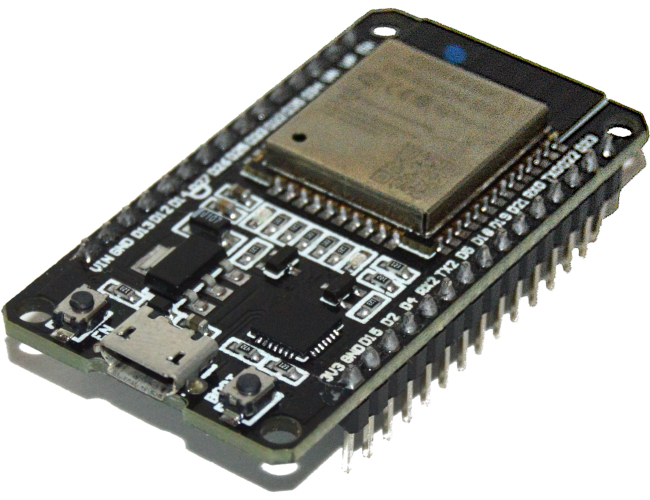
\includegraphics{luanode.png}};
\node (restart)at(0.85,1.85) {};
\node (boot)at(2.25,1){};
\node (regulator)at(1.6,2.3){};
\node (uart)at(2.65, 1.4){};
\node (module)at(3, 3.5){};
\node[left of = boot, node distance=3.5cm] (boot_label) {Bootloader button};
\node[left of = restart, node distance=3.5cm] (restart_label) {Restart button};
\node[left of = regulator, node distance=3.5cm] (regulator_label) {Voltage regulator};
\node[left of = uart, node distance=5cm] (uart_label) {USB to UART chip};
\node[left of = module, node distance=3.5cm] (module_label) {ESP32-WROOM-32D};

\draw[->, orange, ultra thick] (boot_label) -- (boot);
\draw[->, orange, ultra thick] (restart_label) -- (restart);
\draw[->, orange, ultra thick] (regulator_label) -- (regulator);
\draw[->, orange, ultra thick] (uart_label) -- (uart);
\draw[->, orange, ultra thick] (module_label) -- (module);
\end{tikzpicture}
\end{center}

The ESP-IDF (IoT Development Framework) is a library provided by Espressif systems. It integrates into and extends the dedicated hardware provided by the processor.
For example, Writing code against the WiFi transceiver requires using the IDF's TCP, UDP, or HTTP library.
Similarly, cryptography support is provided through the IDF's port of mbedtls, and the SPI flash is exposed through several libraries inside of the IDF.

\subsubsection{SPIFFS}

One particularly useful part of the IDF is SPIFFS (SPI Flash FileSystem).
It exposes a section of the SPI non-volatile flash storage as a basic filesystem.
SPIFFS does not support directories, so a file saved as \texttt{/spiffs/a/b/c.txt} would be in the same directory as \texttt{/spiffs/d.txt}.
SPIFFS also does not support journaling, so if power is removed halfway through a write operation, it must be reformatted.
This means that the ability to restore from a complete format is important.
SPIFFS also limits filenames to 31 characters.

The Nihilo platform hides file I/O behind trees of values, objects and arrays, using JSON files.
The cJson package is included in IDF, and was used for all storage in this project.

\subsubsection{WebAssembly/wasm3}

Although the target of this project is the ESP32, the goal is for it to be architecture agnostic.
This includes both running on different instruction sets and running on different types of computer including desktops and servers.
The problem of targeting different types of device using the same standard is similar to the problem websites were made to solve.
The environment of the web adds the bonus that browser-based runtimes are sandboxed and have been aggressively tested for vulnerabilities.

Javascript, though popular, is a bad fit for creating this platform.
Efficient runtimes are large and are usually themselves very architecture-dependent.
In addition, embedded developers tend to favour strong, static typing and DIY memory management, historically meaning C but a variety of newer languages such as Rust, Golang, and C++ have also been gaining popularity.
Emscripten and later WebAssembly were created to enable C-style languages on the web.
The former compiles code to a highly optimizable subset of Javascript, asm.js, which is backwards compatible with any Javascript engine but runs at near-native speeds in a supported one \cite{asm}.
The latter is an extension to asm.js which abandons the link to Javascript entirely, compiling code to a new instruction set running on an idealised processor \cite{wasm}.

WebAssembly (often shortened to WASM) is intended to be executed using a AOT (ahead of time)  or JIT (just in time) compiler, translating the abstract WASM instructions into real instructions to be executed on the processor.
The difference between JIT and AOT is that AOTs translate into code before the program is run, while JITs compile just before the code is executed.
JITs are generally faster because they can optimize based not just on static analysis but also the actual, runtime values of the variables being used.
Slower than both types of compiler are interpreters, which iterate over the commands one by one and execute them by calling functions associated with each command.
Although compilers are prefereable, they are harder to implement, harder to secure, harder to debug, and require porting to each instruction set they must run on.
Because of WASM's relative immaturity, only two partially implemented runtimes exist for embedded architectures;
\begin{itemize}
\item WebAssembly Micro Runtime (WAMR), the official Bytecode Alliance runtime for running webassembly on microcontrollers.
WAMR can run both in AOT and interpreter mode.
It WAMR is well implemented, but lacks ESP-IDF support and porting the entire runtime is beyond the scope of this project.
\item Wasm3, an unofficial interpreter for WebAssembly. 
Although wasm3 is less professionally implemented, it has excellent support for ESP-IDF.
Its simplicity also aids in modifications and experiments. 
\end{itemize}

Wasm3 was chosen for this project. Prior to running WebAssembly using wasm3, it must be generated. In order to keep the project as a single programming language, C++ was chosen as the source language to compile WebAssembly from.

\subsection{System Design}
\subsubsection{Machines}

The fundamental, indivisible unit of Nihilo is the machine; many machines can be stored on each physical device. Machines are an idealised and abstract version of a computer; communication, execution, and data storage all happen at the machine level. Communication between and within devices happens from one machine to another, using remote procedure calls. Within SPIFFS, each machine is represented by a JSON and WASM file; the JSON storing data and the WASM storing code.

Many machines can be stored on one device, potentially including machines providing self-contained units of functionality developed by third parties. In order to be useful, however, the user must create a single, master machine, tying together all of the others. When the device boots it will connect to WiFi, load the master machine, and execute its \texttt{entry()} function. This can then be used to instantiate functionality in other machines.

\subsubsection{Security Model}

For security purposes, machines are sandboxed from each other, but have absolute power over their internal environment. This is because machines are from a single origin, analogous to how javascript has absolute power over its own HTML under the same origin policy, but can only communicate with others through specific channels. Every machine in Nihilo has an asymmetric keypair. Because every communication in Nihilo has an origin and destination machine, it can be cryptographically verified that;
\begin{itemize}
\item The message was sent only by the stated origin.
\item The message can be read only by the stated destination.
\end{itemize}

RSA (Rivest–Shamir–Adleman)\cite{rsa}, the industry standard algorithm for asymmetric cryptography, was initially considered for this task. Although RSA is very secure, developing for the microcontroller platform exposes a set of issues with RSA which are usually hidden by the power of modern computers. The first of these problems is that key generation (keygen) is profoundly computationally intensive. RSA's hardness assumption is a stronger version of its keygen process; both involving the factorisation of very large numbers. RSA keygen on the ESP32 takes in excess of 20 seconds.

ECC \cite{ecc}(Elliptic Curve Cryptography) is a set of cryptographic primitives based on modular elliptic curves. ECC was built into an asymmetric cryptosystem called ECDH (Elliptic Curve Diffie-Hellman), which is far more computationally efficient than RSA. It has a number of advantages over RSA;
\begin{itemize}
\item Keygen is finished in 200ms, a 100 times speedup.
\item ECDH is not an encryption algorithm, but a key agreement protocol where all of the necessary information is already embedded in the public key of the peer. Both RSA and ECDH need a symmetric encryption algorithm for the bulk exchange of data, but RSA requires a dedicated protocol to send the encrypted symmetric key from one peer to the other while ECDH does not.
\item ECC curve25519 public and private keys are 32 bytes long, as opposed to at least 128 bytes with RSA.
\item Every pair of peers has its own secret, which requires the private key of one and the public key of the other. This negates the need for a dedicated signature, which would be required under RSA.
\end{itemize}

The sum of these advantages is a massively streamlined communication process compared to one implemented using RSA. The 200ms keygen means that machines can be created much faster, while the implicit signature and key exchange negate the need of an SSL-style intermediate layer.

Because the cryptographic verification requires holding the keypair, ownership of the keypair is for all intents and purposes ownership of the machine. The security model breaks down if multiple devices hold the same keypair, so transferring private keys between devices or exposing them to WASM code is \textbf{explicitly forbidden}.

There are two desired capabilities of any asymmetric encryption scheme; security and authentication. Security is the knowledge that only the recipient of the message can decode it. Authentication is the knowledge that the recipient is who they say they are. The ECDH algorithm used by the Nihilo runtime implicitly provides security, but not authentication, which would require one of;

\begin{itemize}
\item A dedicated Public Key Infrastructure (PKI), built on ECC, allowing any claims of identity to be traced back to a common trusted third party.
\item An integration into an existing PKI, such as SSL.
\item A hybrid approach, where trust is rooted in SSL but becomes transferred to Nihilo at some point down the chain to the device attempting to authenticate.
\end{itemize}

Ultimately, the alternative to building a PKI chosen was using the public keys as the primary identifier of a machine. Because there is no known mechanism to efficiently forge a public key, the resulting keys are almost guaranteed to be unique.

Once ECDH has been run, transforming a keypair of one machine and a public key of the other into a shared secret, the message must be symmetrically encrypted. The algorithm chosen was AES\cite{aes}, an efficient block cipher. AES works one block at a time, applying encryption to 16 bytes, then moving on to the next 16 bytes. The original implementation of AES, called ECB mode, had a flaw where identical blocks were encrypted as identical ciphertext, exposing ECB encryption to a variety of attacks, which were rectified with CBC mode. This mode uses the previous block to help encrypt the next, so requires an initialization vector to randomise the first block.

Because the initialization vector is required to decrypt the data, it is included in Nihilo as the 0th block of any encrypted data. If \(x\) is the length of the unencrypted data and b is the block size (16 bytes), the formula for calculating the length of encrypted data is as follows;

\[ ( \lceil x/b \rceil +1) \times b\]

32-byte public keys can be unwieldy, for instance SPIFFS filenames are limited to 31 characters long including extension. In order to simplify this, and to make user interface easier, a 12-byte ID can be used. This is the first 12-bytes of the SHA256 digest of the public key. It is worth noting that while creating a fraudulent key with the same ID is extremely computationally intensive, it is not outside the realm of possibility with future machines, so IDs cannot provide the same security guarantees as public keys. Between devices, Nihilo always uses the full 32 byte public key.

The most important factor in creating a random identifier is minimizing the risk that two entities are randomly assigned the same ID. Poorly engineered identification schemes are vulnerable to a class of exploits known as birthday attacks, in which a forged entity that happens to have the same ID can impersonate the target entity. Thanks to the pigeonhole principle\cite{pigeon}, it is known that any mapping which reduces a large space (all public keys) down to a smaller space (all IDs) must have distinct items in the large space which map to the same item in the small one. In the context of hashing, this is known as a hash collision.

Protecting against a targeted birthday attack, attempting to forge an ID for one specific target, can be achieved with an 8-byte ID, corresponding to a search space \( 2^{8 \times 8} \) hashes wide. If it was possible to check at a rate of 1,000,000 hashes per second, the search space would be exhausted after more than 500,000 years.

It is, however, insufficient to ensure that attackers cannot artificially create a fraudulent ID. The 12-byte length of the ID was not chosen to prevent brute forcing of a \textbf{specific ID}, but to prevent any \textbf{pair of IDs} happening to be identical. This is both more likely on a per-ID basis and happens more often, every time a machine is created on any device. Assuming the hardware random number generator and SHA256 algorithm are both mathematically ideal, the ID space is \( 2^{12 \times 8} \) hashes wide. If \( n \) is the number of assigned hashes, the probability that there exists at least one pair which are the same, \( p \), is approximated by the following formula\cite{birth};

\[ n = \sqrt{2 \times 2^{12 \times 8} \times ln\frac{1}{1-p}}\]

Collision probabilities are given by the following table
\begin{table}[H]
\begin{tabular}{l|l|l}
p				&n							&\( \approx \) equivalent to assigning one hash to \\ \hline
\( 10^{-10}\)	&\( 1.26 \times 10^{10}\)	& every person alive today (\( 7.8 \times 10^{9}\))\\
\( 10^{-7}\)	&\( 1.26 \times 10^{11}\)	& every person who has ever lived (\( 1.09 \times 10^{11}\)) \\
0.01			&\( 3.99 \times 10^{13}\)	& every red blood cell in the human body (\( 2.63 \times 10^{13}\)) \\
0.1				&\( 1.29 \times 10^{14}\)	& every cell in a human body (including bacteria) (\( 10^{14}\))

\end{tabular}
\end{table}

12-byte IDs allow for expansion to tens of trillions of machines before collision becomes an issue, so there is much room for expansion.

\subsection{Implementation}
\subsubsection{Tooling}

There are three major pieces of tooling that were required to implement Nihilo;
\begin{itemize}
\item A pass-through WiFi access point, to streamline network access for the ESP32s
\item A directory server, to facilitate discovery of peers
\item The compiler, programmer, and associated toolchains
\end{itemize}

Allowing for a simple connection to private resources is a common problem in developing open-source software. WiFi credentials, API keys and bitcoin addresses are often left in code which is pushed into public repositories. In order to develop without adding support for Eduroam, and exposing university login details in the code, create\_ap \cite{createap}  was used. This turns WiFi-enabled linux computers into repeaters, taking in one WiFi network while creating another with dependable, specified parameters that can be developed against.

The other component was an HTTP-based directory server, implemented in python. This is simply a public list of known machines, registered using POST requests, and retrieved using GET requests. To simplify handling, the server will only send back machines belonging to other devices. 

On boot, the Nihilo runtime registers owned machines to this service, and queries it for those belonging to other devices. If the runtime decodes a packet from an unknown machine, it will add that to the list.

Wasic++, a clang-based C++ to WebAssembly compiler was used to create the code which the machines can run. This is then run through wasm-opt, which reduces the webassembly's size. Finally, it is run through xxd, which converts the bytes of the optimized wasm into a header file that can be compiled into the runtime. On boot, the runtime writes this into the ESP32's SPIFFS as a .wasm file.

Makefiles were used to unify the different build systems and tools (ESP-IDF uses both ninja and cmake). A single command in the src directory can compile the machine's code into a header file using wasic++, compile the runtime into an xtensa ESP32 executable, program the device, and then execute the program printing any logs to the screen. Makefiles use file modification time to only compile files that have changed, so this process usually completes quickly.

\subsubsection{Adding a simple heap to wasm3}

One serious shortcoming in the wasm3 interpreter, which is not documented in their git repository, is the lack of runtime-allocated memory. The \texttt{void* malloc(size\_t size)} call in which memory is dynamically allocated from the heap, has not been implemented. Although only call-stack based memory is necessary for Turing-completeness, heap-based memory can simplify programming.

Wasm3 allocates memory in 65536 byte pages.
In order to maintain the integrity of the sandbox, accessing memory outside of these pages halts execution, so any implementation of malloc must return a pointer somewhere inside of this page. The Nihilo runtime is built on small functions, which are instantiated, run, and asynchronously instantiate other functions. Each individual function has a very small memory footprint, and each wasm3 runtime exists for a short period of time.

It was decided, as a consequence of the small memory footprint of each function, and the limitations to where memory can be allocated, to reserve page offsets 0x0000 to 0x7FFF (32768 bytes) for the stack, and to reserve offsets 0x8000 to 0xFFFF (32767 bytes) for a heap. Because these pages are cleaned up after a short time, no mechanism for freeing memory was created. A \texttt{uint16\_t} at page offset 0x8000 tracks the amount of allocated heap, and is incremented every time more is allocated. Breaking the Nihilo coding model, and creating highly recursive functions, or functions which allocated and freed a lot of memory, would in turn break this memory allocation scheme.


\subsubsection{Task Queue and Communication}

One problem encountered early on in the development of Nihilo was the limited RAM of the ESP32. This is exacerbated by the fact that ESP-IDF only exposes half of this already constrained RAM as heap, with the other half being reserved for the call stack. There is only enough dynamically allocated RAM for one complete wasm3 runtime, which would seem to exclude the possibility of one runtime calling another, and then using its result in an operation. Encryption, and network communication are both also dependent on the heap. Although external RAM chips do exist for the ESP32, requiring these would break compatibility with most off-the-shelf ESP32 modules.

The solution is to use a FIFO (first in, first out) task queue. This allows WASM function calls to be placed onto the queue as tasks and executed one by one. These tasks may optionally also specify callbacks, placing new tasks onto the queue once execution is complete. Two machines can have an asynchronous 'dialogue' through callbacks without ever loading more than one of them at a time. This model can also be extended to communication if the queue also contains calls to machines on other devices, in which the execution is replaced with encrypting and sending the call.

For simplicity, tasks in Nihilo take exactly one char* parameter (which can be nullptr), and either return a char* value, or return nothing (which is treated as a function that returns nullptr by the runtime).

Tasks are encapsulated within the \texttt{task} struct, containing;
\begin{itemize}
\item Origin public key
\item Destination public key
\item A retry count
\item A pointer to the return value
\item The name of the target function
\item The name of the function to call on success
\item The name of the function to call on failure
\item The parameter to be passed to the function (a null terminated string, immediately following the struct in memory)
\end{itemize}

Because the last four are encrypted for any transmission, they are contained within a struct inside of \texttt{task} called \texttt{wire\_task}. If the task executes successfully, and a success function has been set, a new task will be created. This task will have the return value (if there is any) of the previous task as its parameter, and the on success function as its target. The origin of one task becomes the destination of the next and vice versa.  Failures are treated in the same way, with a description of the error as their parameter.

As with the rest of the runtime, the primary design goal of the Nihilo protocol was simplicity. Nihilo communicates using an encrypted, stateless, single-verb, asynchronous protocol. It is encrypted because every message can only be read by its sender or receiver. It is stateless because messages are not part of a sequence; a connection is made, used to send one message, and then closed. It is single-verb because unlike HTTP, the protocol only knows how to invoke a single type of action; calling a function. It is asynchronous because it does not block until a reply has been received, rather invoking a new function when this happens. Nihilo uses TCP because a high reliability is desired, through Berkeley sockets.

Due to the stateless nature of the protocol, the runtime will only use any individual connection once. It is opened by the origin of the call, the call is sent, and then the connection is terminated. Only incoming connections and other tasks can enqueue tasks, so once the task queue is empty there is nothing to do but listen for connections. This single-threaded approach does have the downside that connections can only be received while the task queue is empty, but a well designed system should be able to work around this flaw.

In order to explore how the runtime communicates, consider the following (An API reference is in the next two sections for specific definitions of individual functions);

Device A has master machine \( x \), with the following code;
\begin{tcolorbox}[colback=white,grow to left by=2.5mm,grow to right by=2.5mm,left*=0mm,right*=0mm,sharp corners]
\begin{verbatim}
NIH_VOID(entry, param){}
NIH_CHARS(RPC, param){
  //write "hello, world" into M.N in persistent JSON
  readString("M.N", "hello, world");
  //read value back out of JSON
  char* ret;
  readString("M.N", &ret);
  return ret;
}
\end{verbatim}
\end{tcolorbox}


Device B has master machine \( y \), with the following code;
\begin{tcolorbox}[colback=white,grow to left by=2.5mm,grow to right by=2.5mm,left*=0mm,right*=0mm,sharp corners]
\begin{verbatim}
NIH_VOID(entry, param){
  unsigned char* ids;
  //find the peer:
  int known = knownPubs(&ids, 0, 1);
  //if the peer is found, call RPC against it
  if(known > 0)
    queue(ids, "RPC", nullptr, "success", "fail");
}
NIH_VOID(success, param){
  logStr("success");
  if(param != nullptr)
    logStr(param);
}
NIH_VOID(fail, param){
  logStr("failure");
  if(param != nullptr)
    logStr(param);
}
\end{verbatim}
\end{tcolorbox}

If A then B is turned on, the following events occur from the perspective of the user;

\begin{enumerate}
\item Directory server is reset.
\item Device A turns on, connects to wifi, and registers its master machine.
\item Machine \( x \) executes its entry function, which is empty.
\item Device B turns on, connects to wifi, and registers its master machine.
\item Machine \( y \) executes its entry function, querying a non-local machine from the runtime, and sending it a call for the \texttt{RPC()} function, with the \texttt{success()} and \texttt{fail()} functions as the possible outcomes of the call. The call has no parameter.
\item Device A receives the call, records the IP address of Machine \( y \) (previously unknown because A turned on before B) and begins to execute \texttt{RPC()}.
\item Device A writes then queries \lq M.N' from machine \( x \)'s persistent JSON storage.
\item Machine \( y \) returns the string to Machine \( x \) by calling the \texttt{success()} function.
\item Device A prints out \lq hello, world'.
\end{enumerate}

If Device B were to encounter a fatal, non-recoverable error in its execution of \texttt{RPC}, it would call \texttt{fail()} instead of \texttt{success()}. Giving too much information in an error message such as the specific exception has been known to create security flaws, including ones that can be used to extract sensitive data \cite{weberror}. For this reason, any error internal to the users code calls the fail handler with the parameter set a generic all-encompassing message, \lq execution error'.

On a lower level, however, this process is more complicated. The code touches communication, encryption, JSON storage, and WASM execution.  Sequence diagrams can be used to help explain registering and querying machines to the directory, which are contained in steps 2 and 4;

\begin{center}
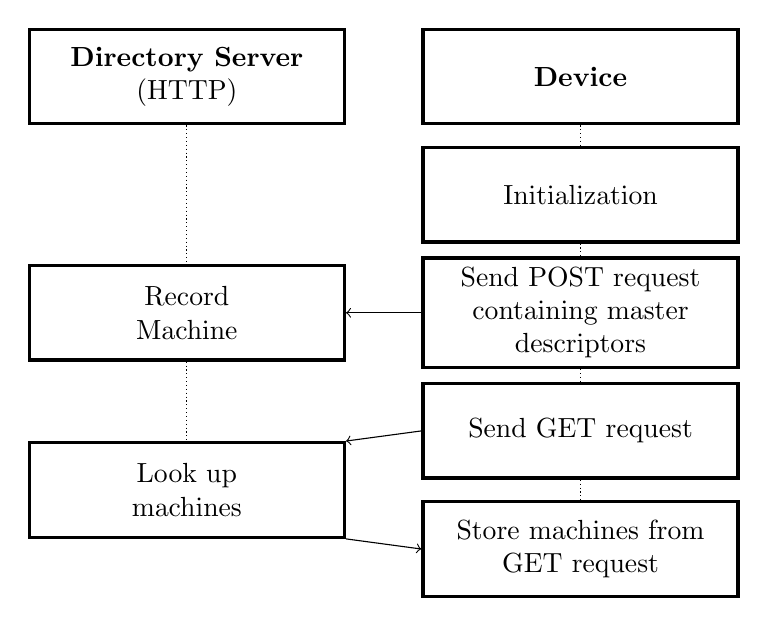
\begin{tikzpicture}[
box/.style={rectangle, draw=black, fill=white, very thick, minimum width=40mm, minimum height=12mm, align=center},
empty/.style=
]
\node[box](dir){\textbf{Directory Server}\\(HTTP)};
\node[box](dev)[right of = dir, node distance=5cm]{\textbf{Device}};
\node[box](init_dev)[below of = dev, node distance=1.5cm]{Initialization};
\node[box](dev_register)[below of = init_dev, node distance=1.5cm]{Send POST request\\containing master\\descriptors};
\node[box](dir_register)[left of = dev_register, node distance=5cm]{Record\\Machine};
\node[box](dev_query_get)[below of = dev_register, node distance=1.5cm]{Send GET request};
\node[empty](dir_get_guide)[left of = dev_query_get, node distance=5cm]{};
\node[box](dir_query_get)[below of = dir_get_guide, node distance=7.5mm]{Look up\\machines};
\node[box](dev_query_receive)[below of = dev_query_get, node distance=1.5cm]{Store machines from\\GET request};

\draw[densely dotted] (dir) -- (dir_register);
\draw[densely dotted] (dev) -- (init_dev);
\draw[densely dotted] (init_dev) -- (dev_register);
\draw[densely dotted] (dir_register) -- (dir_query_get);
\draw[densely dotted] (dev_register) -- (dev_query_get);
\draw[densely dotted] (dev_query_get) -- (dev_query_receive);

\draw[->] (dev_register) -- (dir_register);
\draw[->] (dev_query_get.west) -- (dir_query_get.north east);
\draw[->] (dir_query_get.south east) -- (dev_query_receive.west);

\end{tikzpicture}
\end{center}

The POST request is a machine descriptor, containing the IP address and public key of the target machine in the form \texttt{IP\_ADDR:HEX\_PUBLIC\_KEY}. Only a single machine may be registered at once, but several POSTs may be made to register several machines. If a given machine is re-registered with a new IP address, the old IP address is deleted and the new IP is added instead. Because devices may turn on or off, or lose internet connection, the IP address in the directory may not be the most up to date, and may not work at all. All directory server operations happen on port 80 (the standard HTTP port), and against the root (http://address/) file. Because the directory server gives publicly available information, it is not encrypted with HTTPS.

When a get request is made to the HTTP server, it will collate all known machines not at the requesting device's IP address, and send them to the device. It does this by first sending a count of how many descriptors will be sent, followed by a newline, then the descriptors also separated by newlines;

\texttt{4 \newline
IP\_ADDR:HEX\_PUBLIC\_KEY \newline
IP\_ADDR:HEX\_PUBLIC\_KEY \newline
IP\_ADDR:HEX\_PUBLIC\_KEY \newline
IP\_ADDR:HEX\_PUBLIC\_KEY
}

Steps 5 and 8 involve sending, and 6 and 9 involve receiving messages. Because these messages are encrypted, they have two packets; outer (unencrypted) packets directing them to their destination while providing information required to decrypt them, and inner (encrypted) packets containing the actual function to call. The structure of the outer packet is straightforward;

\begin{table}[H]
\begin{tabular}{|p{25mm}|l|l|p{45mm}|}
\hline
\textbf{Field Name}	& \textbf{Start byte}	& \textbf{End byte}		& \textbf{Description} \\ \hline
Origin Pub					& 0									& 31							& Public Key of origin machine \\ \hline
Destination Pub			& 32								& 63							& Public Key of destination machine \\ \hline
Contents Length			& 63								& 79							& True pre-encryption length of inner packet \\ \hline
Body								& 80								& N								& Encrypted data (first 16 bytes are the Initialization Vector) \\ \hline
\end{tabular}
\end{table}

The first three (Origin and Destination Pub, Contents Length) fields are contained within the \texttt{packet\_header} struct for ease of handling. The only thing that can be told from intercepted packets, without the shared secret, is the message endpoint machines and the message length and frequency. While it may allow an attacker to deduce the general nature of the communication, they should not be able to tell its content. SSL exposes similar information through port numbers and message lengths, and is considered highly secure.

Once the packet has been decrypted, is parsed as an inner packet.

\begin{table}[H]
\begin{tabular}{|p{25mm}|l|l|p{45mm}|}
\hline
\textbf{Field Name}	& \textbf{Start byte}		& \textbf{End byte}		& \textbf{Description} \\ \hline
Destination ID			& 0											& 11									& ID of the target machine. Used to verify packet has been decoded correctly.  \\ \hline
Function name				& 12										& 31									& Name of the function to call. Null-terminated string.  \\ \hline
On Success					& 32										& 51									& Name of the function to call on origin machine if this task completes successfully. Null-terminated string. \\ \hline
On Failure					& 52										& 71									& Name of the function to call on origin machine if this task does not complete successfully. Null-terminated string. \\ \hline
Parameter Null			& 72										& 72									& Is the parameter null? \\ \hline
Parameter						& 73										& N										& Null-terminated parameter \\ \hline
\end{tabular}
\end{table}

Like the outer packet, Function name to Parameter Null are incorporated into a struct for ease of handling. This is called \texttt{wire\_task}, and incorporates all of the information needed to execute the task, other than the origin and destination machine. These public keys, as well as device-specific data are in the \texttt{task} struct. Both \texttt{wire\_task} and \texttt{task} are usually followed directly in memory by the null-terminated parameter if any exists, but this cannot be inside of the struct because it is of varying length.
How these packets are used can also be explained with a sequence diagram. This one covers steps 4 to 9;
\begin{center}
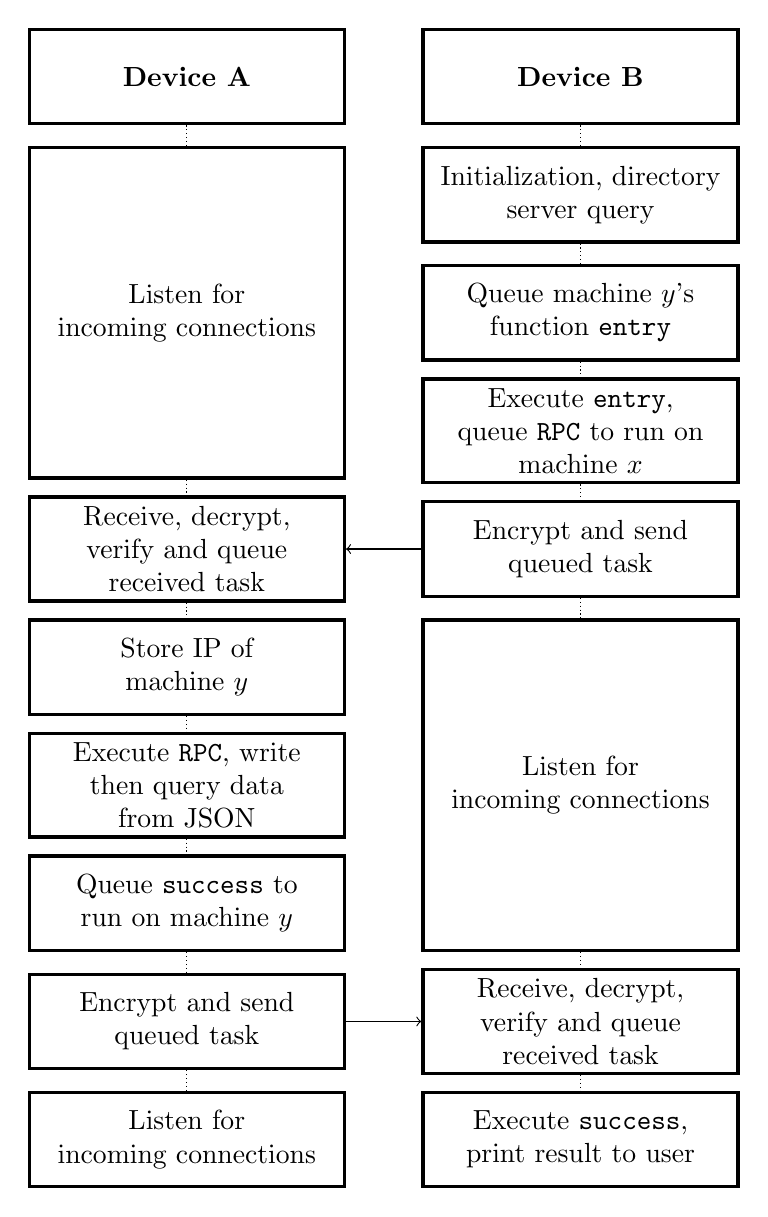
\begin{tikzpicture}[
box/.style={rectangle, draw=black, fill=white, very thick, minimum width=40mm, minimum height=12mm, align=center},
empty/.style=
]
\node[box](a){\textbf{Device A}};
\node[box](b)[right of = a, node distance=5cm]{\textbf{Device B}};

\node[box](b_init)[below of = b, node distance=1.5cm]{Initialization, directory\\server query};
\node[box](b_queue_entry)[below of = b_init, node distance=1.5cm]{Queue machine \( y \)'s\\function \texttt{entry}};
\node[box](b_begin_entry)[below of = b_queue_entry, node distance=1.5cm]{Execute \texttt{entry},\\ queue \texttt{RPC} to run on\\machine \( x \)};
\node[box](b_send_rpc)[below of = b_begin_entry, node distance=1.5cm]{Encrypt and send\\queued task};
\node[box, minimum height = 4.2cm](b_listen)[below of = b_send_rpc, node distance=3cm]{Listen for\\incoming connections};

\node[box, minimum height = 4.2cm](a_pre_listen)[left of = b_queue_entry, node distance=5cm]{Listen for\\incoming connections};
\node[box](a_queue_rpc)[left of = b_send_rpc, node distance=5cm]{Receive, decrypt,\\verify and queue\\received task};
\node[box](a_store_y)[below of = a_queue_rpc, node distance=1.5cm]{Store IP of\\machine \( y \)};
\node[box](a_exec_rpc)[below of = a_store_y, node distance=1.5cm]{Execute \texttt{RPC}, write\\ then query data\\from JSON};
\node[box](a_queue_success)[below of = a_exec_rpc, node distance=1.5cm]{Queue \texttt{success} to\\run on machine \( y \)};
\node[box](a_send_success)[below of = a_queue_success, node distance=1.5cm]{Encrypt and send\\queued task};
\node[box](a_listen)[below of = a_send_success, node distance=1.5cm]{Listen for\\incoming connections};

\node[box](b_queue_success)[right of = a_send_success, node distance=5cm]{Receive, decrypt,\\verify and queue\\received task};
\node[box](b_begin_success)[below of = b_queue_success, node distance=1.5cm]{Execute \texttt{success},\\print result to user};

\draw[densely dotted] (a) -- (a_pre_listen);
\draw[densely dotted] (a_pre_listen) -- (a_queue_rpc);
\draw[densely dotted] (a_queue_rpc) -- (a_store_y);
\draw[densely dotted] (a_store_y) -- (a_exec_rpc);
\draw[densely dotted] (a_exec_rpc) -- (a_queue_success);
\draw[densely dotted] (a_queue_success) -- (a_send_success);
\draw[densely dotted] (a_send_success) -- (a_listen);


\draw[densely dotted] (b) -- (b_init);
\draw[densely dotted] (b_init) -- (b_queue_entry);
\draw[densely dotted] (b_queue_entry) -- (b_begin_entry);
\draw[densely dotted] (b_begin_entry) -- (b_send_rpc);
\draw[densely dotted] (b_send_rpc) -- (b_listen);
\draw[densely dotted] (b_listen) -- (b_queue_success);
\draw[densely dotted] (b_queue_success) -- (b_begin_success);

\draw[->] (b_send_rpc) -- (a_queue_rpc);
\draw[->] (a_send_success) -- (b_queue_success);

\end{tikzpicture}
\end{center}

Device A stores machine \( y \)'s IP address and public key when the task is received, because device A turns on before B. Because the directory server is only queried by the Nihilo runtime when the device boots, device A has no knowledge of device B or machine \( y \) until it receives the first packet. Device B does not do the same when it receives its message because it already knows about machine \( x \).
\subsection{Nihilo API}
\subsubsection{Nihilo API Macros}

\textbf{\texttt{NIH\_VOID(NAME, PARAMNAME)}}\newline
Create a new Nihilo-exposed function with name \texttt{NAME}, and a \texttt{const char*} parameter called \texttt{PARAMNAME}. Replaces the normal function declaration. If it is called with no parameter, \texttt{PARAMNAME} will equal \texttt{nullptr}.

\begin{tcolorbox}[colback=white,grow to left by=2.5mm,grow to right by=2.5mm,left*=0mm,right*=0mm,sharp corners]
\begin{verbatim}
NIH_VOID(entry, param){
  logStr("hello, world!);
}
\end{verbatim}
\end{tcolorbox}

\textbf{\texttt{NIH\_CHARS(NAME, PARAMNAME)}}\newline
Same as \texttt{NIH\_VOID(NAME, PARAMNAME)}, but returns a \texttt{const char *}.

\begin{tcolorbox}[colback=white,grow to left by=2.5mm,grow to right by=2.5mm,left*=0mm,right*=0mm,sharp corners]
\begin{verbatim}
NIH_CHARS(entry, param){
  return "hello, world.";
}
\end{verbatim}
\end{tcolorbox}

\textbf{\texttt{WASM\_IMPORT(MODULE,NAME)}}\newline
Internal macro, assisting with exposing functions to the user.

\subsubsection{Nihilo API Functions}

\textbf{\texttt{void mallocWasm(void** target, uint32\_t size)}}\newline
Replacement for malloc(). Pointer pointed to by \texttt{target} is is set to point to a new buffer of length \texttt{size} bytes. Allocates heap inside of wasm3's memory space.

\begin{tcolorbox}[colback=white,grow to left by=2.5mm,grow to right by=2.5mm,left*=0mm,right*=0mm,sharp corners]
\begin{verbatim}
NIH_VOID(entry, param){
  char* buf;
  mallocWasm((void**)&buf, 50);
  strcpy(buf, "test");
  logStr(buf);
}
\end{verbatim}
\end{tcolorbox}

\textbf{\texttt{void writeString(const char* path, const char* value)}}\newline
Saves \texttt{value} in \texttt{path} in the current machine's JSON. Only objects and strings are currently supported to save, and only strings to directly edit, delineated by full stops(\texttt{.}). If the write is under an object that doesn't yet exist, it will create that object.

\begin{tcolorbox}[colback=white,grow to left by=2.5mm,grow to right by=2.5mm,left*=0mm,right*=0mm,sharp corners]
\begin{verbatim}
NIH_VOID(save_value, param){
  writeString("M.N.C.Str", param);
}
\end{verbatim}
\end{tcolorbox}

\textbf{\texttt{void readString(const char* path, char** target)}}\newline
Looks up \texttt{path} in the current machine's JSON. Pointer pointed to by \texttt{target} is set to point to the value read out of JSON.

\begin{tcolorbox}[colback=white,grow to left by=2.5mm,grow to right by=2.5mm,left*=0mm,right*=0mm,sharp corners]
\begin{verbatim}
NIH_VOID(log_value, param){
  char* val;
  readString("M.N.C.Str", &val);
  if(val != nullptr)
    logStr(val);
}
\end{verbatim}
\end{tcolorbox}

\textbf{\texttt{int knownPubs(unsigned char** IdsOut, int include\_local, int include\_non\_local)}}\newline
Lists machines currently known to this device. if \texttt{include\_local} is set to 0, machines on the device will be excluded from the list. Similarly, if \texttt{include\_non\_local} is set to 0, machines not on the device will be excluded. \texttt{IdsOut} is set to point to a list of the 32-byte public keys of the requested devices, and the function returns the number of machines which have been included in \texttt{IdsOut}.

\begin{tcolorbox}[colback=white,grow to left by=2.5mm,grow to right by=2.5mm,left*=0mm,right*=0mm,sharp corners]
\begin{verbatim}
NIH_VOID(log_value, param){
  unsigned char* ids;
  int known = knownPubs(&ids, 0, 1);
  if(known > 0)
    logStr("Devices knows of non-local machines");
}
\end{verbatim}
\end{tcolorbox}

\textbf{\texttt{void logStr(const char* tolog)}}\newline
Log a string to the user, using the ESP-IDF monitoring program.

\begin{tcolorbox}[colback=white,grow to left by=2.5mm,grow to right by=2.5mm,left*=0mm,right*=0mm,sharp corners]
\begin{verbatim}
NIH_VOID(log_value, param){
  logStr("hello, world");
}
\end{verbatim}
\end{tcolorbox}

\textbf{\texttt{void queue(const unsigned char* target\_pub, const char* fname, const char* param, const char* onsuccess, const char* onfail)}}\newline
Add a new task to the back of the queue, to be executed after every other task currently on the queue. The task will be sent to \texttt{target\_pub}, either directly if it is on this device, or through an encrypted socket if it is on another. If \texttt{target\_pub} is nullptr, it will be sent to the current machine. The target device will execute \texttt{fname(param)}, and pass its result to \texttt{onsuccess} in this machine if it is a success, or \texttt{onfail if not}. \texttt{param}, \texttt{onsuccess} and \texttt{onfail} may be set to \texttt{nullptr}, but \texttt{fname} must be a valid string.

\begin{tcolorbox}[colback=white,grow to left by=2.5mm,grow to right by=2.5mm,left*=0mm,right*=0mm,sharp corners]
\begin{verbatim}
NIH_VOID(entry, param){
  queue(nullptr, "test", "hello!", "success", nullptr);
}
NIH_CHARS(test, param){
  logStr(param);
  return "response";
}
NIH_VOID(success, param){
  logStr(param);
}
\end{verbatim}
\end{tcolorbox}
This example prints;
\begin{tcolorbox}[colback=white,grow to left by=2.5mm,grow to right by=2.5mm,left*=0mm,right*=0mm,sharp corners]
\begin{verbatim}
hello!
response
\end{verbatim}
\end{tcolorbox}

\textbf{\texttt{uint64\_t uptime()}}\newline
Returns the number of milliseconds since the system booted.

\begin{tcolorbox}[colback=white,grow to left by=2.5mm,grow to right by=2.5mm,left*=0mm,right*=0mm,sharp corners]
\begin{verbatim}
NIH_VOID(log_value, param){
  logStr("uptime:");
  logStr(decstr((int)uptime()));
}
\end{verbatim}
\end{tcolorbox}

\textbf{\texttt{char* decstr(int input)}}\newline
Returns the string version of the passed integer, allocated into a new buffer.

\begin{tcolorbox}[colback=white,grow to left by=2.5mm,grow to right by=2.5mm,left*=0mm,right*=0mm,sharp corners]
\begin{verbatim}
NIH_VOID(log_value, param){
  logStr(decstr(5));//prints 5
}
\end{verbatim}
\end{tcolorbox}

\textbf{\texttt{int strdec(char* input)}}\newline
Returns the integer corresponding to the passed string.

\begin{tcolorbox}[colback=white,grow to left by=2.5mm,grow to right by=2.5mm,left*=0mm,right*=0mm,sharp corners]
\begin{verbatim}
NIH_VOID(log_value, param){
  if(strdec(param) == 0) 
    logStr("passed zero");
  else
    logStr("passed non-zero");
}
\end{verbatim}
\end{tcolorbox}

\textbf{\texttt{void setReturn (const char* ret)}}\newline
Internal function, assisting with returning data to the runtime.

\textbf{\texttt{void getParam(char** param)}}\newline
Internal function, assisting with passing the parameter from the runtime to WASM code.

\section{Testing and Results}

In section 5.1, the high-level requirements are listed. There are two types of requirements, \textbf{must} and \textbf{should}. \textbf{Must} level requirements do not require much experimental setup, only a single verification. \textbf{Should} level requirements, on the other hand, are more relative and require experimental parameters to be set beforehand.
\subsection{Execution}
\begin{enumerate}
\item \textbf{Must} suport mature languages, compilers and tooling. This is a fact of the design of Nihilo, and so does not need to be tested.
\item \textbf{Should} execute tasks quickly. It should take under 5 milliseconds (ms) to create an execution context, execute a function, clean up the memory, and then move on to the next task. It will be calculated by taking the time between the start and end logs of the following code, averaging over 10 runs, and dividing by 100:
\begin{tcolorbox}[colback=white,grow to left by=2.5mm,grow to right by=2.5mm,left*=0mm,right*=0mm,sharp corners]
\begin{verbatim}
NIH_VOID(test, param){
  if(strlen(param) > 0) logStr("end");
}
NIH_VOID(entry, param){
  logStr("started");
  for(int i = 0; i < 100; i++){
    char* arg = (char*)(i==99?"end":"");
  queue(nullptr, "test", arg, nullptr, nullptr);
  }
}
\end{verbatim}
\end{tcolorbox}

The results are as follows:
\begin{table}[H]
\begin{tabular}{|l|l|l|l|}
\hline
Start Time(ms)		&End Time(ms)		&100 Task Time(ms)		&Single Task Time(ms)		\\ \hline
2137							&2537						&400    							&4\\ \hline
2627							&3057						&430	    						&4.3\\ \hline
5657							&6067						&410		    					&4.1\\ \hline
2127							&2527						&400			    				&4\\ \hline
3127							&3547						&420				    			&4.2\\ \hline
2147							&2557						&410					    		&4.1\\ \hline
2147							&2557						&410						    	&4.1\\ \hline
2147							&2567						&420						    	&4.2\\ \hline
2177							&2597						&420							    &4.2 \\ \hline
\end{tabular}
\end{table}
\emph{Note:the fact that the 100 task time is always a multiple of 10ms appears to come from periodic buffering in the ESP32's logging system. While this likely affects the results, it is insignificant compared to even the smallest result, \( \pm\)2.5\%.}

The average of the single task times is 4.13 ms, beating the minimum requirement by almost 20\%.

\end{enumerate}
\subsection{Storage}
\begin{enumerate}
\item \textbf{Must} be able to save strings while the device is off. This is proven as a part of tests 3 and 4.
\item \textbf{Must} be able to structure the saved data. This does not need to be tested, as the structure of the saved data is an implicit part of the design.
\item \textbf{Should} write the data quickly.
\item \textbf{Should} read the data quickly.
\end{enumerate}

\subsection{Communication}
\begin{enumerate}
\item \textbf{Must} ensure messages arrive as they are sent. This does not need testing, as it is a part of the TCP protocol, which is assumed to work.
\item \textbf{Must} allow the user to call a function on the target device, using a
string as a parameter and as the return value. This is also an implicit part of the design, which is tested as a part of 4 and 5.
\item \textbf{Must} be secure, the content of a message should not be visible to
an attacker. This cannot be proven, only disproven. If many researchers cannot find a flaw, but a single researcher can, the content of the message is visible to an attacker. All that can be used for this heading is an assurance that the code was tested and audited thoroughly.
\item \textbf{Should} be low-latency, sending a message and receiving a reply
quickly.
\item \textbf{Should} be stable over long periods of time.
\end{enumerate}

\section{Analysis and Conclusion}


\section{Reflection}

\section{Glossary}


\section{References}
\begin{thebibliography}{9}
\bibitem{internetofsh}
  \url{https://www.zdnet.com/article/smart-iot-home-hubs-vulnerable-to-remote-code-execution-attacks/}
\bibitem{32datasheet}
	\url{https://www.espressif.com/sites/default/files/documentation/esp32_datasheet_en.pdf}
\bibitem{lx6datasheet}
	\url{https://mirrobo.ru/wp-content/uploads/2016/11/Cadence_Tensillica_Xtensa_LX6_ds.pdf}
\bibitem{asm}
	\url{http://asmjs.org/spec/latest/}
\bibitem{wasm}
	\url{https://webassembly.github.io/spec/core/_download/WebAssembly.pdf}
\bibitem{rsa}
	\url{https://people.csail.mit.edu/rivest/Rsapaper.pdf}
\bibitem{ecc}
	\url{https://www.ams.org/journals/mcom/1987-48-177/S0025-5718-1987-0866109-5/S0025-5718-1987-0866109-5.pdf}
\bibitem{aes}
	\url{https://nvlpubs.nist.gov/nistpubs/FIPS/NIST.FIPS.197.pdf}
\bibitem{createap}
	\url{https://github.com/oblique/create_ap}
\bibitem{birth}
	\url{http://www.winlab.rutgers.edu/comnet2/Reading/documents/Birthday_attack.pdf}
\bibitem{pigeon}
	\url{https://www.math.ust.hk/~mabfchen/Math391I/Pigeonhole.pdf}
\bibitem{weberror}
  \url{https://owasp.org/www-community/Improper_Error_Handling}
\bibitem{dsa}
  \url{http://iot-dsa.org/get-started/how-dsa-works}
\end{thebibliography}
\end{document}
